%%%%%%%%%%%%%%%%%%%%%%%%%%%%%%%%%%%%%%%%%%%%%%%%%%%%%%%%%%%%%%%%%%%%%%
%     File: ExtendedAbstract_resul.tex                               %
%     Tex Master: ExtendedAbstract.tex                               %
%%%%%%%%%%%%%%%%%%%%%%%%%%%%%%%%%%%%%%%%%%%%%%%%%%%%%%%%%%%%%%%%%%%%%%

\section{Experiments}
\label{sec:experiments}

This section presents a comprehensive experimental evaluation of Aerial-D that spans model training, cross-dataset generalization, and targeted ablations. We first describe the model architecture and training setup, then report cross-dataset results on established aerial referring expression segmentation datasets. Beyond aggregate performance, we also include: (i) ablation of expression enhancement strategies; (ii) ablation of historic-filter training; and (iii) qualitative comparison across language models (o3, base Gemma3, and our distilled Gemma3-Aerial model), coupled with a cost analysis of these alternatives.

\subsection{Model Architecture}
\label{subsec:model_architecture}

In selecting the architecture for our experiments, we prioritized a model that can interpret natural-language descriptions while producing pixel-accurate masks in aerial scenes. Generic segmentation systems rarely meet both requirements under the domain shift of remote sensing, where objects are small, repetitive, and densely arranged. We therefore adopt RSRefSeg as our backbone for referring expression segmentation: it pairs a strong language–image encoder (SigLIP2) with a state-of-the-art mask decoder (SAM), enabling robust semantic grounding alongside precise mask generation. As in the original RSRefSeg training, the model is fine‑tuned via LoRA adapters; we retain this recipe when adapting to the remote‑sensing domain. This choice is further supported by the strong performance reported for RSRefSeg on RRSIS-D\cite{liu2024rotated}, providing a proven baseline for aerial referring expression segmentation and reducing risk in our evaluation.

Concretely, we implement the RSRefSeg architecture\cite{chen2025rsrefseg} in PyTorch, as illustrated in Figure~\ref{fig:rsrefseg_arch}. The design couples SigLIP2\cite{siglip2} for vision–language encoding with SAM\cite{sam} for mask generation. Following the original authors, training uses LoRA (Low‑Rank Adaptation)\cite{lora} adapters inserted into the SAM image encoder and into SigLIP2’s vision and text encoders, while preserving the strong pretraining of these backbones. In practice, adapters are placed on the query and value projection layers in the vision encoders and on the query, key, value, and output projection layers in the text encoder.

\subsection{Experimental Setup}
\label{subsec:experimental_setup}

Our training configuration uses a batch size of 4 with gradient accumulation steps of 2, achieving an effective batch size of 8 samples. The model employs \texttt{SigLIP2-SO400M} for vision–language encoding and \texttt{SAM-ViT-Large} for mask generation when training the combined model. Consistent with the RSRefSeg training strategy, we employ LoRA with rank \(r=32\) for parameter‑efficient adaptation. Training uses AdamW optimizer\cite{adamw} with initial learning rate of 1e-4, weight decay of 0.01, and polynomial learning rate decay with power factor 0.9. Mixed-precision computation and gradient clipping with maximum norm of 1.0 ensure training stability. Inputs are prepared per backbone: images are resized to 384×384 for SigLIP2 and to 1024×1024 for SAM. The historic filters described in Section~\ref{subsec:historic_filters} are incorporated during data preparation for the four non‑historic datasets (Aerial‑D, RRSIS‑D, NWPU‑Refer, RefSegRS): for each dataset, we randomly select 20\% of training images and replace them with a single filtered copy, sampling one of the three filters uniformly for each selected image.

In order to prevent Aerial-D from overwhelming the combined training mix, we limit its contribution to the \emph{Unique Expressions Only} split identified in the ablation below. This choice keeps the total number of Aerial-D samples closer to the scale of the four public datasets—each of which contributes only tens of thousands of expressions—while still exposing the model to the richer cues that the unique-only subset provides. We train the resulting combined model on Aerial-D (unique-only), RRSIS-D\cite{liu2024rotated}, NWPU-Refer\cite{yang2024large}, RefSegRS\cite{yuan2023rrsis}, and Urban1960SatSeg\cite{hao2025urban1960satseg}, and evaluate on their validation splits (Aerial-D uses the \emph{combined-all} validation set). To probe robustness to historical degradations, we additionally evaluate historic-filtered counterparts obtained by converting 100\% of validation images for the four non-historic datasets (Aerial-D, RRSIS-D, NWPU-Refer, RefSegRS) using the three filters from Section~\ref{subsec:historic_filters}. We report these results under the "Hist." columns.

\subsection{Evaluation Results}
\label{subsec:evaluation_results}

Table~\ref{tab:combined_training_results} reports validation results for a single combined model trained jointly on all datasets and evaluated on each dataset's validation split. We present Pass@0.5/0.7/0.9 (shown as IoU@0.5/0.7/0.9 in the table), which measure the percentage of instances whose predicted mask attains IoU greater than or equal to the threshold. We also report two aggregate overlap scores: mIoU, the mean of per-instance IoU values, and oIoU, the overall IoU obtained by summing intersections and unions across all instances before taking their ratio.

The "Hist." columns simply reference the historic-filter validation splits introduced earlier, allowing us to read performance on both versions of each dataset without rehashing the setup.

Quantitatively, the combined model attains strong results across benchmarks. On RRSIS-D, it delivers Pass@0.5/0.7/0.9 of 69.48\%/53.62\%/21.78\% together with 61.70\% mIoU and 73.44\% oIoU; the historic split for the same dataset stays close at 58.35\% mIoU and 71.73\% oIoU. On NWPU-Refer, the model records 40.53\%/27.65\%/8.45\% alongside 37.89\% mIoU and 51.34\% oIoU, while the filtered imagery yields 31.52\% mIoU and 46.17\% oIoU. On RefSegRS, the evaluation reports 41.30\%/9.05\%/2.09\%, 40.10\% mIoU, and 45.05\% oIoU, with the historic variant tapering to 32.79\% mIoU and 36.74\% oIoU. On Urban1960SatSeg, which already comprises historic photography, the model reaches 78.05\%/59.96\%/28.25\% together with 69.35\% mIoU and 87.27\% oIoU. Despite the diversity of expression styles and object categories across datasets, these scores match or surpass the author‑reported baselines for the four public benchmarks. For Aerial‑D, we further establish baseline performance in terms of mIoU and oIoU, providing a reference point for future work on this dataset.

% Combined training performance table
\begin{table*}[t]
\centering
\caption{Combined Training Performance Evaluation - Model Trained on All Dataset Train Sets (Historic-filtered results in \textcolor{blue}{blue})}
\label{tab:combined_training_results}
\begin{tabular}{@{}lcccccccc@{}}
\toprule
\textbf{Dataset} & \textbf{IoU@0.5} & \textbf{IoU@0.7} & \textbf{IoU@0.9} & \multicolumn{2}{c}{\textbf{mIoU}} & \multicolumn{2}{c}{\textbf{oIoU}} \\
\cmidrule(lr){5-6} \cmidrule(lr){7-8}
 & & & & \textbf{Orig.} & \textbf{Hist.} & \textbf{Orig.} & \textbf{Hist.} \\
\midrule
Aerial-D & 60.10\% & 43.95\% & 13.05\% & 49.78\% & \textcolor{blue}{46.82\%} & 63.44\% & \textcolor{blue}{61.12\%} \\
RRSIS-D & 69.48\% & 53.62\% & 21.78\% & 61.70\% & \textcolor{blue}{58.35\%} & 73.44\% & \textcolor{blue}{71.73\%} \\
NWPU-Refer & 40.53\% & 27.65\% & 8.45\% & 37.89\% & \textcolor{blue}{31.52\%} & 51.34\% & \textcolor{blue}{46.17\%} \\
RefSegRS & 41.30\% & 9.05\% & 2.09\% & 40.10\% & \textcolor{blue}{32.79\%} & 45.05\% & \textcolor{blue}{36.74\%} \\
Urban1960SatSeg & 78.05\% & 59.96\% & 28.25\% & 69.35\% & N/A & 87.27\% & N/A \\
\bottomrule
\end{tabular}
\end{table*}

\subsection{Expression Enhancement Ablation}
\label{subsec:ablation_studies}

In order to quantify how much the enhanced expressions improve segmentation outcomes, we revisit Aerial-D with a controlled experiment. The combined model in Section~\ref{subsec:evaluation_results} blends rule-based descriptions with LLM rewrites, which makes it difficult to isolate the specific contribution of each expression type when comparing against the original, simpler phrasing. We therefore retrain RSRefSeg on Aerial-D with a lighter setup—SAM-ViT-Base replaces SAM-ViT-Large to accelerate the runs, and the LoRA rank is lowered to \(r=16\) while keeping all other optimizer settings, learning schedules, and preprocessing identical to Section~\ref{subsec:experimental_setup}. This configuration keeps the focus on the language differences rather than architectural changes.

Using this setup, we train four separate models, each exposed to a distinct slice of Aerial-D: (i) \emph{Rule-based Only} retains the original deterministic descriptions produced by the rule system; (ii) \emph{Enhanced Only} relies on LLM rewrites that diversify the wording while preserving the target; (iii) \emph{Unique Expressions Only} selects LLM augmentations that inject alternative visual cues; and (iv) \emph{Combined All} unites the three sources. Figure~\ref{fig:llm_enhancement_example} illustrates how the enhanced variants expand the phrasing beyond the rule-based baseline. We evaluate the resulting checkpoints on four validation sets without additional tuning: Aerial-D (using the \emph{combined-all} validation split) and three external datasets—RefSegRS, RRSIS-D, and NWPU-Refer—to observe how each expression type supports generalization beyond the training distribution.

Table~\ref{tab:ablation_expression_types} summarizes the results and explicitly reports both the number of \emph{Samples} and \emph{Epochs} used per configuration. Looking across datasets, several consistent patterns emerge. On Aerial-D, the \emph{Combined All} configuration achieves the best accuracy, which is expected given that the validation distribution matches that training mixture. For the three external datasets, different subsets yield the strongest generalization: on RRSIS-D, varying the language (\emph{Enhanced Only}) helps most; on NWPU-Refer, emphasizing varied visual cues (\emph{Unique Expressions Only}) is most beneficial; and on RefSegRS, a combination of both types provides the best results. These outcomes highlight the breadth of ways to phrase referring expressions and show that leveraging LLMs to introduce targeted variety improves cross-dataset generalization.

In order to keep early stopping responsive to each subset, we monitor validation loss across the four runs and halt training as soon as it begins to rebound. Because the \emph{Combined All} subset is roughly three times larger than the others, its validation loss ticks upward immediately after the second epoch, so we stop that run at two epochs. The three smaller subsets continue improving through the fourth epoch before showing the same rise, allowing four full passes over their data. This schedule means that the language-variation and unique-only models actually process fewer total samples than the combined run, yet they surpass it on RRSIS-D and NWPU-Refer. The outcome reveals that curated expression subsets can be more sample efficient than the full mixture, which is why the combined model in Section~\ref{subsec:evaluation_results} draws on the unique-only split of Aerial-D. Beyond sample efficiency, constraining Aerial-D to that subset keeps the cross-dataset mix from being dominated by a single corpus whose expression pool would otherwise reach into the millions.

% Ablation expression types table with explicit epochs and samples
\begin{table*}[t]
\centering
\caption{Expression Enhancement Ablation Across Four Datasets}
\label{tab:ablation_expression_types}
\resizebox{\textwidth}{!}{%
\begin{tabular}{@{}lcc|cc|cc|cc|cc@{}}
\toprule
\multirow{2}{*}{\textbf{Training Configuration}} & \multirow{2}{*}{\textbf{Samples}} & \multirow{2}{*}{\textbf{Epochs}} & \multicolumn{2}{c|}{\textbf{Aerial-D}} & \multicolumn{2}{c|}{\textbf{RefSegRS}} & \multicolumn{2}{c|}{\textbf{RRSIS-D}} & \multicolumn{2}{c}{\textbf{NWPU-Refer}} \\
\cmidrule(lr){4-5} \cmidrule(lr){6-7} \cmidrule(lr){8-9} \cmidrule(lr){10-11}
 & & & % \textbf{Pass@0.7} & 
\textbf{mIoU} & \textbf{oIoU} & % \textbf{Pass@0.7} & 
\textbf{mIoU} & \textbf{oIoU} & % \textbf{Pass@0.7} & 
\textbf{mIoU} & \textbf{oIoU} & % \textbf{Pass@0.7} & 
\textbf{mIoU} & \textbf{oIoU} \\
\midrule
Rule-based Only & 371K & 4 & % 26.81\% & 
34.57\% & 39.31\% & % 2.55\% & 
3.73\% & 0.55\% & % 29.89\% & 
34.22\% & 36.46\% & % 13.62\% & 
16.78\% & 13.70\% \\
Enhanced Only & 364K & 4 & % 36.39\% & 
46.45\% & 56.99\% & % \textbf{3.02\%} & 
5.75\% & 4.99\% & % \textbf{35.63\%} & 
\textbf{41.63\%} & \textbf{42.48\%} & % \textbf{16.90\%} & 
21.89\% & 16.68\% \\
Unique Expressions Only & 382K & 4 & % 35.75\% & 
46.54\% & 63.02\% & % 2.55\% & 
18.32\% & 8.37\% & % 20.86\% & 
31.78\% & 33.73\% & % 15.91\% & 
\textbf{24.68\%} & \textbf{29.22\%} \\
Combined All & 1,118K & 2 & % \textbf{39.54\%} & 
\textbf{49.33\%} & \textbf{64.30\%} & % 1.86\% & 
\textbf{18.80\%} & \textbf{8.58\%} & % 23.39\% & 
34.07\% & 34.80\% & % 15.91\% & 
24.57\% & 28.27\% \\
\bottomrule
\end{tabular}%
}
\end{table*}

\subsection{Distillation Ablation: Gemma3 vs. o3 Model Comparison}
\label{subsec:distillation_ablation}

This ablation measures how the generator choice inside the LLM enhancement stage affects expression quality and overall cost. We evaluate three options for producing the enhanced expressions: OpenAI’s o3, the off‑the‑shelf Gemma3‑12B, and the distilled Gemma3-Aerial model described in Section~\ref{subsec:llm_expression_generation} (see Figure~\ref{fig:llm_distillation}).

All three models are prompted and decoded in the same way so that differences stem from the generator rather than the interface. The base Gemma3 baseline frequently hallucinates objects that are not present, which undermines segmentation training. Distillation sharply reduces those errors, producing grounded descriptions that resemble the o3 outputs while remaining accessible on local hardware.

Table~\ref{tab:cost_comparison} quantifies the practical impact. Running o3 across \(\sim\)300{,}000 targets would cost roughly \$6.2K, whereas the distilled Gemma3 produces comparable guidance for about \$26—roughly 238× cheaper because inference runs locally instead of via a commercial API. Figure~\ref{fig:distillation_comparison} illustrates why the student is worth training: the base Gemma3 hallucinates a second baseball diamond that does not exist, while the distilled variant stays aligned with the image and mirrors the grounded detail that o3 provides.

% Cost comparison table
\begin{table}[t]
\centering
\caption{Cost Analysis: Gemma3 vs. o3 Model for Large-Scale Annotation\protect\footnotemark}
\label{tab:cost_comparison}
\resizebox{\columnwidth}{!}{%
\begin{tabular}{@{}lcc@{}}
\toprule
\textbf{Model} & \textbf{Cost per request} & \textbf{Cost for 300K requests} \\
\midrule
o3 Model & \$0.020728 & \$6,218.32 \\
Distilled Gemma3 & \$0.000087 & \$26.01 \\
\midrule
\textbf{Savings} & \textbf{238× cheaper} & \textbf{\$6,192.31 (99.6\%)} \\
\bottomrule
\end{tabular}%
}
\end{table}
\footnotetext{Cost calculations based on API pricing — o3: \$2.00 per million input tokens, \$8.00 per million output tokens (OpenAI API platform); Gemma3-12B: \$0.035 per million input tokens, \$0.141 per million output tokens (OpenRouter inference provider). Average tokens per request: o3 (1,670.8 input, 2,173.3 output), Gemma3 (1,330.0 input, 284.7 output). Calculations based on 15 sample requests.}

\begin{figure*}[t]
\centering
\begin{minipage}{0.5\textwidth}
\centering
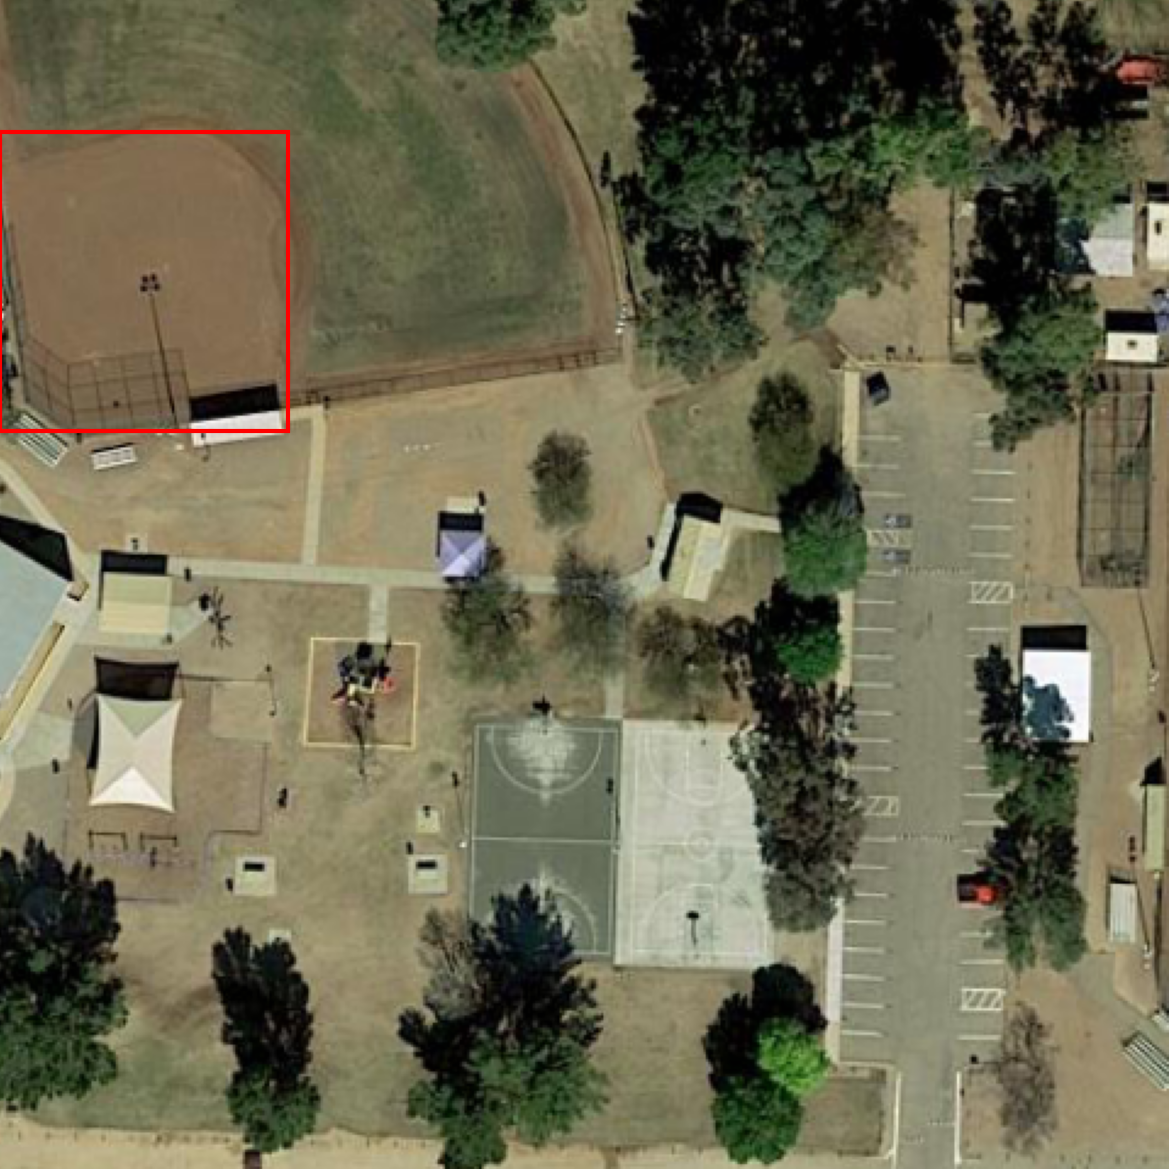
\includegraphics[width=0.65\textwidth]{./images/3llm.png}
\end{minipage}%
\begin{minipage}{0.5\textwidth}
\centering
\hspace{-1cm}
\raisebox{-0.3\height}{%
\footnotesize
\begin{tabular}{@{}p{2cm}p{5cm}@{}}
\toprule
\textbf{Expression Type} & \textbf{Example} \\
\midrule
Original & the orange baseball diamond in the top left \\
\midrule
o3 Enhanced & the orange baseball diamond with the light pole near home plate in the upper left \\
\midrule
Gemma3 Base & the bright orange baseball diamond to the left of another similar baseball diamond in the top left \\
\midrule
Gemma3-Aerial-12B & the orange baseball field with a chainlink fence surrounded by grass to the north and trees to the west \\
\bottomrule
\end{tabular}%
}
\end{minipage}
\caption{Qualitative comparison between o3, vanilla Gemma3 base model, and our fine-tuned Gemma3-Aerial-12B model on aerial imagery. The table shows how each model enhances the original rule-based expression using an identical prompt and decoding setup, demonstrating the progression from basic rule-based descriptions through increasingly capable LLM enhancements.}
\label{fig:distillation_comparison}
\end{figure*}


\subsection{Historic Filter Ablation Study}
\label{subsec:historic_ablation}

In order to understand how much the historic-image filters described in Section~\ref{subsec:historic_filters} contribute to robustness, we repeat the combined training without injecting those filters. Models that only encounter clean, contemporary imagery typically falter when historic photographs suddenly introduce monochrome toning, contrast loss, or sepia casts. We therefore run an ablation that removes the filters from the training mix and compares the resulting model against the full recipe.

Table~\ref{tab:historic_ablation_results} summarizes this experiment. We keep the same architecture, optimization settings, and five-dataset mixture used for the main combined model (Aerial-D unique-only, RRSIS-D, NWPU-Refer, RefSegRS, and Urban1960SatSeg), but we stop replacing 20\% of the training images in Aerial-D, RRSIS-D, NWPU-Refer, and RefSegRS with filtered counterparts. In other words, every sample those datasets contribute during this ablation arrives exactly as stored, whereas the main model receives a uniformly sampled black-and-white, film-grain, or sepia transformation for one fifth of their images.

We use the same format as in Table~\ref{tab:combined_training_results}: each dataset is scored on its original validation split, and the "Hist." columns again transform 100\% of the Aerial-D, RRSIS-D, NWPU-Refer, and RefSegRS validation images using the three filters from Section~\ref{subsec:historic_filters} uniformly. Because the ablated model encounters these degradations for the first time at validation, the clean columns climb a few points while the historic columns respond unevenly: RRSIS-D and NWPU-Refer remain resilient, whereas RefSegRS still sheds about five points of mIoU. This behavior indicates that the filter injections mainly protect datasets whose semantics become ambiguous once contrast and color cues are suppressed.

% Historic filter ablation table
\begin{table*}[t]
\centering
\caption{Historic Filter Ablation Study — Combined model trained on all datasets without historic-filter augmentation}
\label{tab:historic_ablation_results}
\resizebox{\textwidth}{!}{%
\begin{tabular}{@{}lcccccccc@{}}
\toprule
\textbf{Dataset} & \textbf{IoU@0.5} & \textbf{IoU@0.7} & \textbf{IoU@0.9} & \multicolumn{2}{c}{\textbf{mIoU}} & \multicolumn{2}{c}{\textbf{oIoU}} \\
\cmidrule(lr){5-6} \cmidrule(lr){7-8}
 & & & & \textbf{Orig.} & \textbf{Hist.} & \textbf{Orig.} & \textbf{Hist.} \\
\midrule
Aerial-D & 59.48\% (\textcolor{red}{-0.62}) & 43.37\% (\textcolor{red}{-0.58}) & 12.60\% (\textcolor{red}{-0.45}) & 49.21\% (\textcolor{red}{-0.57}) & \textcolor{blue}{43.57\%} (\textcolor{red}{-3.25}) & 62.88\% (\textcolor{red}{-0.56}) & \textcolor{blue}{58.14\%} (\textcolor{red}{-2.98}) \\
RRSIS-D & 74.60\% (\textcolor{darkgreen}{+5.12}) & 58.39\% (\textcolor{darkgreen}{+4.77}) & 20.75\% (\textcolor{red}{-1.03}) & 64.36\% (\textcolor{darkgreen}{+2.66}) & \textcolor{blue}{59.02\%} (\textcolor{darkgreen}{+0.67}) & 75.59\% (\textcolor{darkgreen}{+2.15}) & \textcolor{blue}{72.50\%} (\textcolor{darkgreen}{+0.77}) \\
NWPU-Refer & 46.02\% (\textcolor{darkgreen}{+5.49}) & 32.32\% (\textcolor{darkgreen}{+4.67}) & 10.66\% (\textcolor{darkgreen}{+2.21}) & 41.06\% (\textcolor{darkgreen}{+3.17}) & \textcolor{blue}{33.42\%} (\textcolor{darkgreen}{+1.90}) & 58.35\% (\textcolor{darkgreen}{+7.01}) & \textcolor{blue}{53.04\%} (\textcolor{darkgreen}{+6.87}) \\
RefSegRS & 47.33\% (\textcolor{darkgreen}{+6.03}) & 13.23\% (\textcolor{darkgreen}{+4.18}) & 1.16\% (\textcolor{red}{-0.93}) & 41.31\% (\textcolor{darkgreen}{+1.21}) & \textcolor{blue}{27.73\%} (\textcolor{red}{-5.06}) & 50.30\% (\textcolor{darkgreen}{+5.25}) & \textcolor{blue}{32.21\%} (\textcolor{red}{-4.53}) \\
Urban1960SatSeg & 78.46\% (\textcolor{darkgreen}{+0.41}) & 60.98\% (\textcolor{darkgreen}{+1.02}) & 28.66\% (\textcolor{darkgreen}{+0.41}) & 69.81\% (\textcolor{darkgreen}{+0.46}) & N/A & 87.80\% (\textcolor{darkgreen}{+0.53}) & N/A \\
\bottomrule
\end{tabular}%
}
\end{table*}

Values in parentheses denote percentage-point change relative to the baseline combined model in Table~\ref{tab:combined_training_results}, with \textcolor{red}{red} marking drops and \textcolor{darkgreen}{green} marking gains.
